\documentclass[a4paper,10pt,twocolumn]{article}
\usepackage[T1]{fontenc}
\usepackage[utf8]{inputenc}
\usepackage[italian]{babel}
\usepackage[top=2.5cm, bottom=2.5cm, left=2.5cm, right=2.5cm]{geometry}
\usepackage{graphicx}
\graphicspath{{/home/egg/uni/root/RootSimulation/build/analysis/}}
\usepackage{amsmath}
\usepackage{booktabs}
\usepackage{caption}
\captionsetup[table]{position=top}
\captionsetup[figure]{position=bottom}
\usepackage{dblfloatfix}
\usepackage[hidelinks]{hyperref}

\title{Relazione ROOT}
\author{Nicolò Montalti}
\date{\today}

\begin{document}
\maketitle
\section{Introduzione}
Il programma si divide in due parti: una di generazione e una di analisi. Durante la generazione vengono generati $10^5$ gruppi di 100 particelle secondo proporzioni predefinite. Per ogni generazione vengono riempiti degli istogrammi con
In seguito gli istogrammi vengono analizzati, disegnati su delle canvas e salvati.

\section{Struttura del codice}
Alla base del programma ci sono tre classi: ParticleType, ResonanceType e Particle. La classe ParticleType contiene la massa, la carica e il nome di ogni tipo di particella. Dispone inoltre dei rispettivi getters e di un metodo Print che permette di stampare a schermo ogni informazione. La classe ResonanceType eredita da ParticleType, secondo la relazione "is-a", e aggiunge la larghezza di risonanza con il rispettivo getter. Sovrascrive inoltre il metodo Print, in modo da stampare anche quest'ultimo attributo. Si è scelto di fare ereditare ResonanceType da ParticleType in quanto ogni particella di risonanza possiede tutti gli attributi di una particella canonica (nome, massa e carica), ma non è vero il contrario.

La classe Particle aggiunge le proprietà cinematiche tipiche di una particella fisica, cioè le tre componenti della quantità di moto. Dato che ogni particella è caratterizzata unicamente dal tipo e dalla quantità di moto, si è scelto di non fare ereditare Particle da ParticleType. Se si fosse sfruttata l'ereditarietà, per ogni istanza di Particle sarebbero stati salvati in memoria nome, massa e carica, sprecando risorse. Si è quindi preferito includere nella classe Particle un array statico di puntatori ParticleType e un indice intero. L'array è riempito tramite il metodo statico AddParticleType e per ogni istanza di Particle viene assegnato un valore all'indice per indicare il tipo di particella.

Oltre ai canonici getters e setters, Particle dispone di un metodo Decay2Body che permette ai $K^*$ di decadere in un pione e in un kaone di carica opposta. Il decadimento conserva

\section{Generazione}
Inizialmente vengono generati $10^5$ eventi di 100 particelle secondo le proporzioni definite in tab.~\ref{tab:proporzioni} attraverso un blocco if-else. La quantità di moto è assegnata estraendone il modulo da una distribuzione esponenziale di media 1 e gli angoli polare e azimutale da due distribuzioni uniformi. Le particelle $K^*$ vengono fatte decadere con pari probabilità in un $\pi^+$ e in un $K^-$ o in $\pi^-$ e in un $K^+$.

\begin{table*}
  \caption{Particelle generate dal programma con le rispettive proporzioni}
  \label{tab:proporzioni}
  \centering
  \begin{tabular}{cccc}
    \toprule
    Particelle         & Carica (e) & Simbolo & Percentuale \\
    \midrule
    Pioni              & +1         & $\pi^+$ & 40\%        \\
    Pioni              & -1         & $\pi^-$ & 40\%        \\
    Kaoni              & +1         & $K^+$   & 5\%         \\
    Kaoni              & -1         & $K^-$   & 5\%         \\
    Protoni            & +1         & $p^+$   & 4.5\%       \\
    Protoni            & -1         & $p^-$   & 4.5\%       \\
    Kaoni di risonanza & 0          & $K^*$   & 1\%         \\
    \bottomrule
  \end{tabular}
\end{table*}

\section{Analisi}

\begin{table*}
  \caption{Abbondanza delle particelle generate}
  \label{tab:abbondanza}
  \centering
  \begin{tabular}{cccc}
    \toprule
    Specie  & Occorrenze osservate $(10^5)$ & Occorrenze attese $(10^5)$ \\
    \midrule
    $\pi^+$ & 39.99 $\pm$ 0.02              & 40                         \\
    $\pi^-$ & 39.99 $\pm$ 0.02              & 40                         \\
    $K^+$   & 5.000 $\pm$ 0.007             & 5.0                        \\
    $K^-$   & 5.004 $\pm$ 0.007             & 5.0                        \\
    $p^+$   & 4.504 $\pm$ 0.007             & 4.5                        \\
    $p^-$   & 4.507 $\pm$ 0.007             & 4.5                        \\
    $K^*$   & 0.998 $\pm$ 0.003             & 1.0                        \\
    \bottomrule
  \end{tabular}
\end{table*}


\begin{table*}
  \caption{Fit delle distribuzioni}
  \label{tab:fit}
  \centering
  \begin{tabular}{cccccc}
    \toprule
    Variabile           & Distribuzione & Parametro del fit          & $\chi^2$ & DOF & $\chi^2$ / DOF \\
    \midrule
    Angolo azimutale    & pol0          & $(10000 \pm 3) \cdot 10^2$ & 27.86    & 9   & 3.10           \\
    Angolo polare       & pol0          & $(10000 \pm 3) \cdot 10^2$ & 15.20    & 9   & 1.70           \\
    Modulo dell'impulso & expo          & 1.0002 $\pm$ 0.0003        & 20.48    & 18  & 1.14           \\
    \bottomrule
  \end{tabular}
\end{table*}

\begin{table*}
  \caption{Analisi dei decadimenti delle $K^*$}
  \label{tab:fit}
  \centering
  \begin{tabular}{p{5cm}cccc}
    \toprule
    Distribuzione gaussiana                                                                          & Media                 & Sigma ($10^{-2}$) & Ampiezza ($10^4$) & $\chi^2$ / DOF \\
    \midrule
    Massa invariante ottenuta da differenza delle combinazioni $\pi K$ di carica discorde e concorde & 0.90101 $\pm$ 0.00017 & 4.536 $\pm$ 0.011 & 2.072 $\pm$ 0.008 & 78.7           \\
    \midrule
    Massa invariante ottenuta dalla differenza delle combinazioni di carica discorde e concorde      & 0.89110 $\pm$ 0.00016 & 4.227 $\pm$ 0.011 & 2.016 $\pm$ 0.009 & 77.2           \\
    \midrule
    Massa invariante ottenuta dalle vere $K^*$                                                       & 0.89167 $\pm$ 0.00016 & 5.042 $\pm$ 0.011 & 1.316 $\pm$ 0.005 & 0.855          \\
    \bottomrule
  \end{tabular}
\end{table*}

\begin{figure*}
  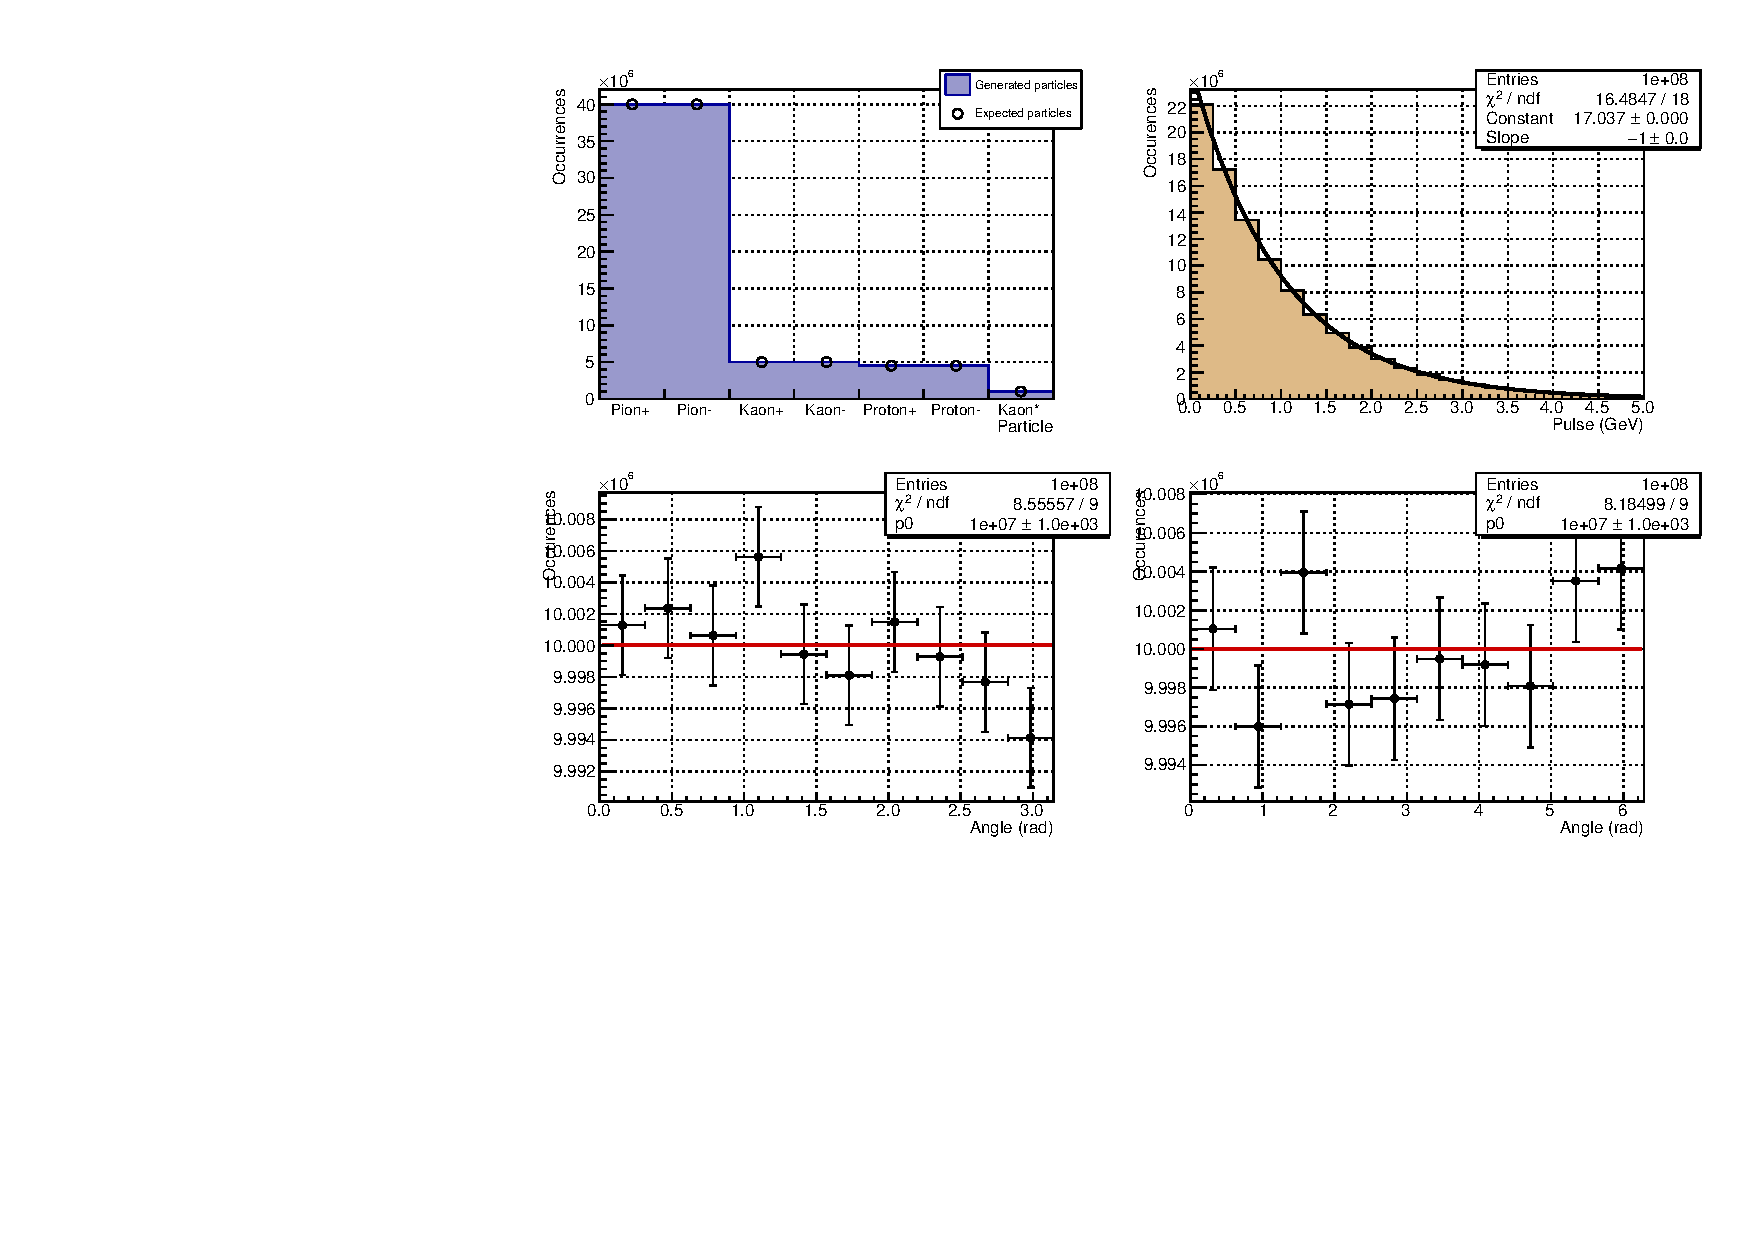
\includegraphics[width=0.95\linewidth]{Generation.pdf}
  \caption{Istogrammi delle particelle generate e attese (in alto a sx), del modulo dell'impulso con fit esponenziale (in alto a dx) e degli angoli azimutali e polari con fit pol0 (in basso)}
  \label{fig:Generation}
\end{figure*}

\begin{figure*}
  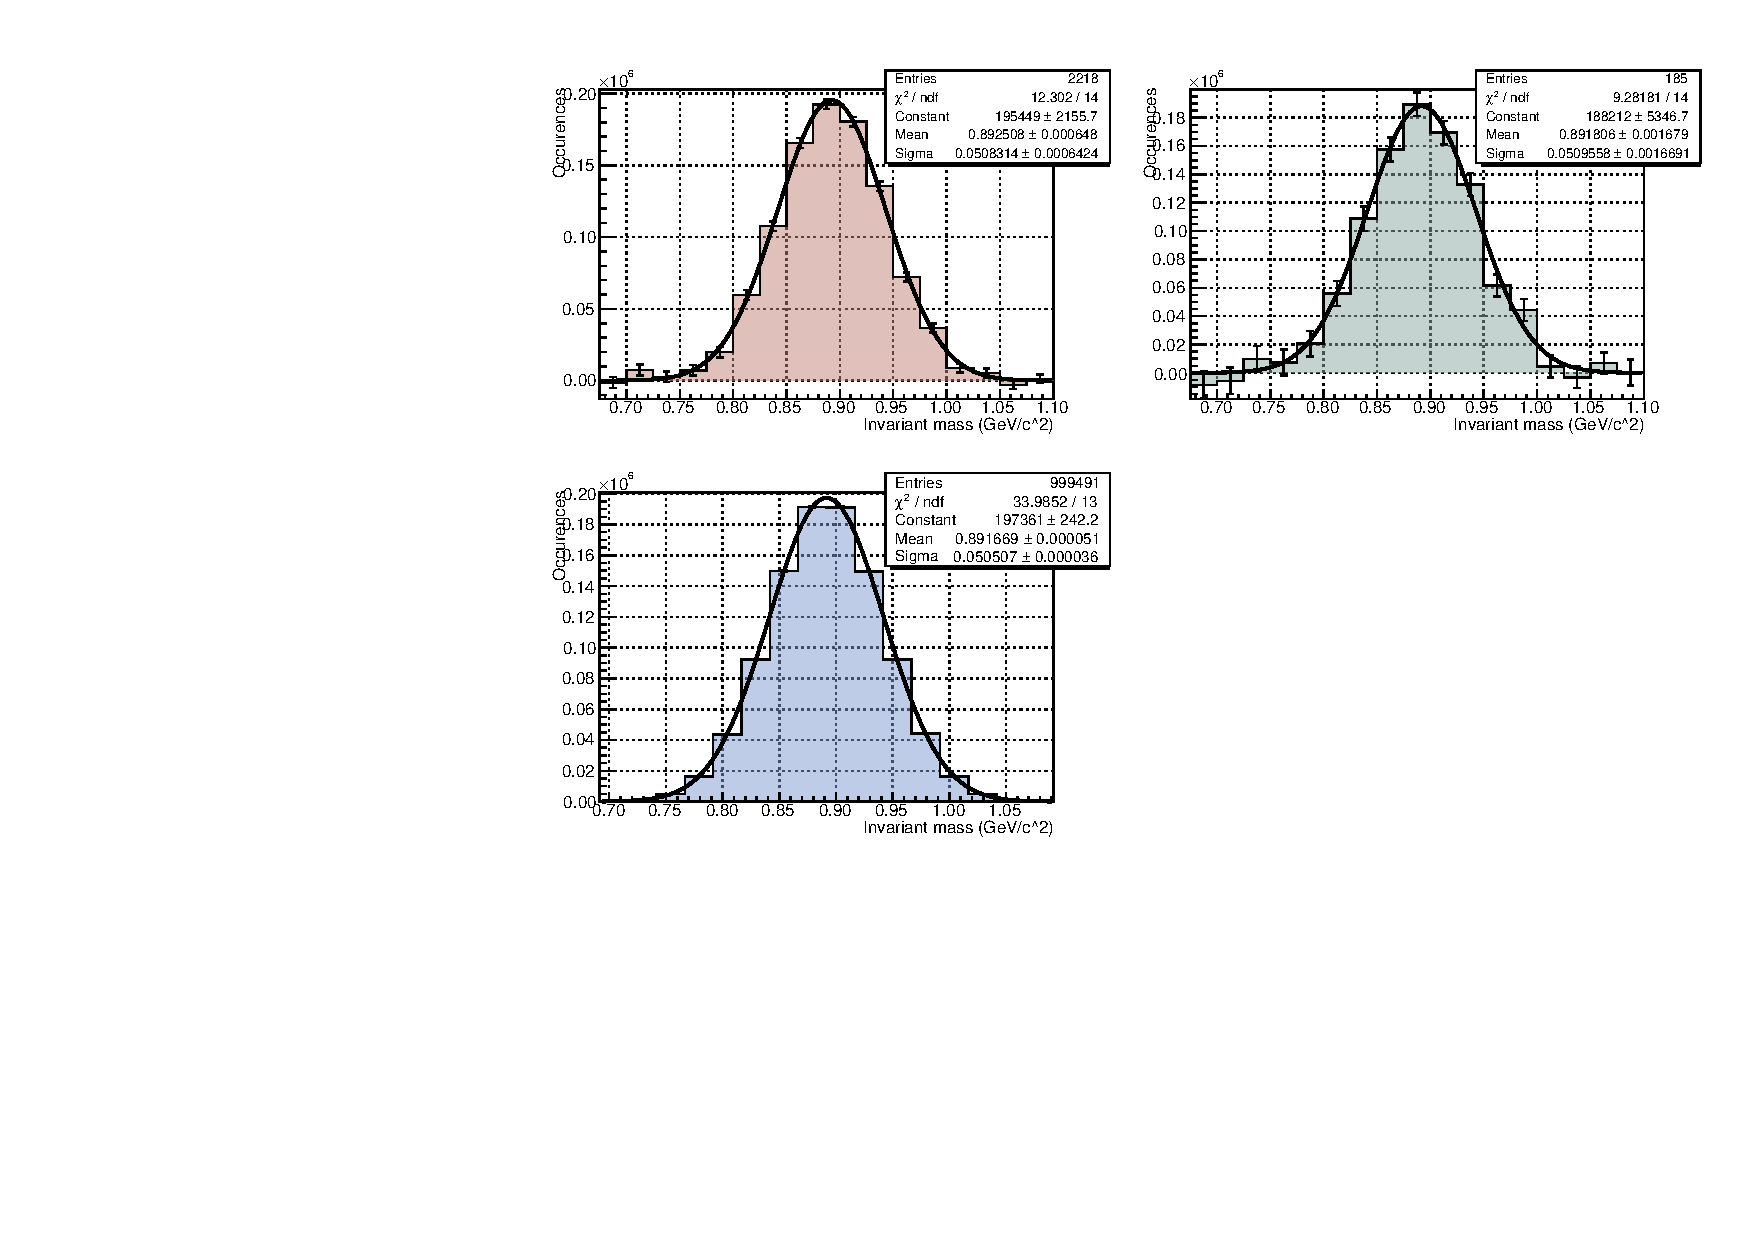
\includegraphics[width=0.95\linewidth]{InvMass.pdf}
  \caption{Istogrammi della massa invariante ottenuta rispettivamente dalla differenza delle combinazioni $k\pi$ di carica uguale ed opposta (in alto a sx), dalla differenza di combinazioni di particelle di carica uguale ed opposta (in alto a dx) e dalle coppie $K\pi$ generate nei decadimenti delle $K^*$ (in basso a sx)}
  \label{fig:InvMass}
\end{figure*}

\end{document}
